
\chapter{Oscillazioni smorzate e forzate}
\section{Introduzione}

Oggetto di questa ricerca è lo studio delle oscillazioni smorzate e forzate di un pendolo. Studiando il variare delle oscillazioni al variare della frequenza operativa della forzante, si studierà il fenomeno della risonanza.

\begin{wrapfigure}[24]{R}{0.28\textwidth}
  \begin{center}
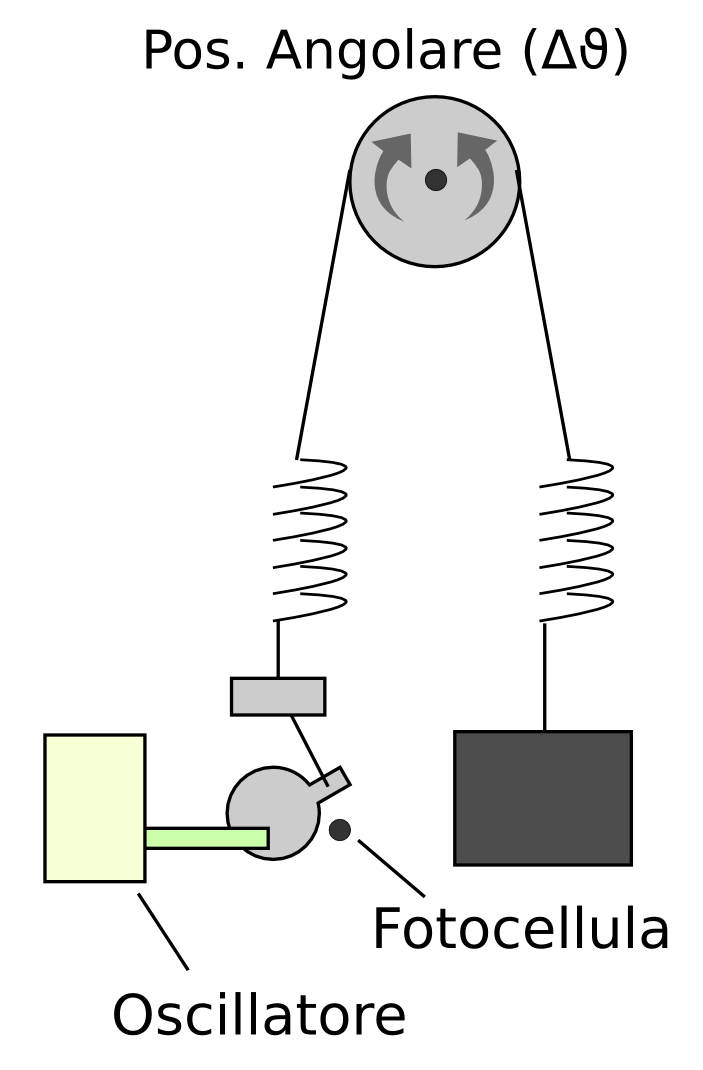
\includegraphics[scale=0.7]{../grafici/oscillazioni-schema.png}
  \end{center}
  \caption*{Schema dell'esperimento}
\end{wrapfigure}

\subsection{Strumenti}
\begin{center}
\begin{tabular}{l|l}
Strumento & Precisione\\
\midrule
Calibro & $\pm 0.05$ mm\\ 
Sensore di rotazione & $\pm 0.00157$ rad\\ 
Alimentatore & $\pm 0.01$ V\\ 

\end{tabular}
\end{center}
L'attrezzatura utilizza è costituita da un disco metallico fissato ad una puleggia. La puleggia è messa in oscillazione da un filo alle cui estremità vi sono un oscillatore  elettromeccanico, che agisce come forzante, e un sistema di due molle. Al disco è possibile avvicinare e allontanare un magnete, che ha la funzione di smorzare il moto.

\section{Oscillazioni libere}

Si pone in oscillazione il disco, con l'oscillatore elettromeccanico spento e il magnete posizionato sufficientemente lontano, in modo da non influenzare il moto della puleggia. Un sensore di posizione misura lo spostamento angolare; il sensore è collegato ad un computer, ed il programma DataStudio traccia in tempo reale il grafico dello spostamento angolare in funzione del tempo. Si interpolano dunque i dati con una funzione sinusoidale per determinare il periodo, e si ricava: $$T=1.47\pm0.02\ s$$ L'errore riportato è quello che il programma stesso attribuisce alla rilevazione, ed è determinato dalla precisione degli strumenti di rilevamento e dall'interpolazione dei dati.\\
Dal periodo possiamo ricavare il valore della pulsazione $\omega$, dalla relazione:
\begin{equation}\label{omepe}
\omega=\frac{2\pi}{T}
\end{equation}
e si ottiene:
$$\omega=4.272 \pm \sigma_\omega\ rad/s$$
con un errore dato dalla propagazione di quello su $T$:
$$\sigma_{\omega}= \left|\frac{-2\pi}{T^2}\right| \sigma_T=0.06\ rad/s$$
\section{Oscillazioni smorzate}

Si avvicina il magnete al disco metallico; nello specifico dei dati ora riportati è stato avvicinato di 4.80 mm. Il moto oscillatorio risulterà così smorzato per effetto delle correnti di Focault, e seguirà la legge:
\begin{equation}\label{eq:thetat}
\theta (t) = A_0 e^{- \gamma t} \sin(wt+\phi)+\theta_0
\end{equation}
I dati riportati sono stati ottenuti con due interpolazioni differenti. Per ricevere il valore del periodo si è usata una funzione sinusoidale; invece per determinare ampiezza ($A_0$), coefficiente di smorzamento ($\gamma$), pulsazione ($\omega$), costante di fase ($\phi$) e spostamento iniziale ($\theta_0$) si è fatto uso della \ref{eq:thetat}.\footnote{L'incertezza ricavata in questo modo è diversi ordini di grandezza più piccola rispetto al dato interpolato, e da qui in avanti sarà considerata trascurabile. Adotteremo questa convenzione per tutte le incertezze che incontreremo nel resto dell'esperimento.}

A questo punto, noti $\omega$ e $\gamma$, è possibile calcolare $ \omega_0 $, cioè la pulsazione per le oscillazioni libere, tramite l'equazione:
\begin{equation}
\omega = \sqrt{\omega_0^2 - \gamma^2}
\end{equation}
da cui:
\begin{equation}\label{eq:omega}
\omega_0 = \sqrt{\omega^2 + \gamma^2}
\end{equation}
In particolare, nel caso di sistema meno smorzato, ovvero con il magnete a 4.80 mm:
$$\omega_0=4.275\ rad/s$$

Confrontandolo con il valore che avevamo ricavato interpolando direttamente il grafico delle oscillazioni libere si nota che i due non coincidono; quello misurato dal periodo delle oscillazioni libere è minore di quello ricavato dalla formula: tale discrepanza è dovuta al fatto che si sta lavorando con un sistema reale, dunque tra le sue parti sono presenti degli attriti che smorzano le oscillazioni.

\subsubsection{Magnete a 4.80 mm}
\begin{center}
\begin{tabular}{c c}

\begin{tabular}{c}
$T_{smorzate}=0.145\ s$\\
\\
(da \ref{eq:omega}) $\omega_{0} = 4.275\ rad/s$\\
\end{tabular}

& \hspace{2cm}

\begin{tabular}{c}
$A_0 = 3.08 \pm 0.020\ rad$\\
\\
$\gamma =  0.197 \pm 0.0019\ m^4/kg $\\
\\
$\omega = -4.27  \pm 0.0019\ rad/s $\\
\\
$\phi =  1.93 \pm 0.0069\ rad $ \\
\\
$\theta_0 = -1.53 \pm 0.0019\ rad $\\
\end{tabular}

\end{tabular}

\end{center}

\subsubsection{Magnete a 2.80 mm}
\begin{center}

\begin{tabular}{c c}

\begin{tabular}{c}
$T_{smorzate}=0.877\ s$\\
\\
(da \ref{eq:omega}) $\omega_{0} = 4.297\ rad/s$\\
\end{tabular}

& \hspace{2cm}

\begin{tabular}{c}
$A_0 = 3.4 \pm 0.020\ rad$\\
\\
$\gamma =  0.636 \pm 0.0057\ m^4/kg $\\
\\
$\omega = -4.25  \pm 0.0064\ rad/s $\\
\\
$\phi =  2.38 \pm 0.0076\ rad $ \\
\\
$\theta_0 = -0.57 \pm 0.0038\ rad $\\
\end{tabular}

\end{tabular}

\end{center}

\subsubsection{Magnete a 1.00 mm}

\begin{center}

\begin{tabular}{c c}

\begin{tabular}{c}
$T_{smorzato}=2.15\ s$\\
\\
(da \ref{eq:omega}) $\omega_{0} = 4.291\ rad/s $\\
\end{tabular}

& \hspace{2cm}

\begin{tabular}{l}

$A_0 = 18600 \pm 1300\ rad$ \\
\\
$\gamma= 1.50 \pm 0.0011\ m^4/kg$\\
\\
$\omega = 4.02 \pm 0.0077\ rad/s$\\
\\
$\phi =  26.3 \pm 0.0046 \ rad/s$ \\
\\
$\theta_0 = 0.055 \pm 0.0016\ rad$ \\
\end{tabular}

\end{tabular}

\end{center}

\section{Oscillazioni smorzate-forzate}

Mantenendo il magnete vicino al disco, abbiamo messo in azione l'oscillatore elettromeccanico, che fornisce la componente forzante. Variando il voltaggio dell'alimentatore, la frequenza di rotazione dell'oscillatore cambia: abbiamo così cercato la frequenza di risonanza del sistema.
Poiché il periodo di oscillazione della puleggia coincide con quello della forzante (dopo un certo tempo), abbiamo potuto leggere direttamente il periodo dal valore restituito dalla fotocellula. Dopo aver atteso che il sistema si fosse stabilizzato, abbiamo interpolato i dati con il programma DataStudio, secondo la funzione
\begin{equation} \label{A}
A(\omega) = \frac{M_0}{\sqrt{ ({\omega_0}^2-\omega^2)^2 + 4\gamma^2\omega^2}}
\end{equation}

e, misurando l'ampiezza $A(\omega)$, abbiamo ricavato i valori corrispondenti ai parametri liberi $M_0$, $\gamma$ e $\omega_0$. 

Tale procedura è stata ripetuta spostando il magnete a distanze differenti dal disco.
\\
Di seguito sono riportati i dati raccolti e i rispettivi grafici. In tabella sono trascritti i valori dei periodi della forzante (e dunque anche del sistema), il corrispondente $\omega$ (dato dall'equazione \ref{omepe}), e il valore dell'ampiezza dell'oscillazione ottenuto tramite interpolazione con una funzione sinusoidale. Di fianco alle tabelle si trovano i valori ottenuti dall'interpolazione con la funzione \ref{A}. Il grafico illustra l'andamento dell'ampiezza al variare della pulsazione: i picchi corrispondono alla condizione di risonanza.

\subsubsection{Magnete a 4.80 mm}

\begin{center}

\begin{tabular}{c c}

\begin{tabular}{c | c | c}
\textbf{Ampiezza ($rad$)} & \textbf{Periodo ($s$)} & \textbf{Pulsazione ($rad/s$)}\\
\midrule
0.89 & 5.45 & 1.15\\
0.94 & 4.78 & 1.31\\
1.05 & 3.57 & 1.75\\
1.09 & 3.19 & 1.97\\
1.30 & 2.46 & 2.55\\
1.30 & 2.59 & 2.42\\
1.84 & 2.06 & 3.05\\
1.91 & 1.90 & 3.31\\
3.42 & 1.70 & 3.69\\
6.35 & 1.59 & 3.95\\
1.19 & 1.14 & 5.51\\
\end{tabular}

& \hspace{1cm} 

\begin{tabular}{c}
$ \omega_0 = 4.25\ rad/s $\\
\\
$ \gamma = 0.193\ s^{-1}$\\
\\
$ M_0 = 15.3\ s$\\
\end{tabular} 

\end{tabular}

\end{center}
 
\begin{center}

\includegraphics[scale=0.75]{"../grafici/Magnetea48mm"}


\end{center}
 
 
\subsubsection{Magnete a 2.80 mm}
\begin{center}

\begin{tabular}{c c}

\begin{tabular}{c | c | c}
\textbf{Ampiezza} ($rad$) & \textbf{Periodo} ($s$) & \textbf{Pulsazione} ($rad/s$)\\
\midrule
1.68 & 2.00 & 3.14\\
2.95 & 1.63 & 3.85\\
3.22 & 1.44 & 4.36\\
2.17 & 1.30 & 4.83\\
1.20 & 1.15 & 5.46\\
1.67 & 1.24 & 5.06\\
0.99 & 1.10 & 5.71\\
0.68 & 0.98 & 6.40\\
0.51 & 0.89 & 7.06\\
0.26 & 0.74 & 8.49\\
\end{tabular}

& \hspace{1cm}

\begin{tabular}{c}
$ \omega_0 = 4.26\ rad/s $\\
\\
$ \gamma = 0.543\ s^{-1} $\\
\\
$ M_0 = 15.6\ s$\\
\end{tabular}

\end{tabular}

\end{center}

\begin{center}
\includegraphics[scale=0.75]{"../grafici/Magnetea28mm"}

\end{center}


\subsubsection{Magnete a 1.00mm}

\begin{center}

\begin{tabular}{c c}

\begin{tabular}{c | c | c}

\textbf{Ampiezza} ($rad$) & \textbf{Periodo} ($s$) & \textbf{Pulsazione} ($rad/s$)\\
\midrule
1.33 & 2.01 & 3.12\\
1.42 & 1.85 & 3.39\\
1.45 & 1.67 & 3.76\\
1.18 & 1.31 & 4.79\\
1.31 & 1.39 & 4.52\\
1.47 & 1.54 & 4.07\\
0.76 & 1.09 & 5.76\\
0.88 & 1.19 & 5.28\\
1.01 & 1.22 & 5.15\\
0.49 & 0.93 & 6.75\\
0.65 & 1.03 & 6.10\\
0.39 & 0.85 & 7.39\\

\end{tabular}

& \hspace{1cm}

\begin{tabular}{c}
$\omega_0 = 4.37\ rad/s $\\
\\
$\gamma = 1.40 \pm 0.14\ s^{-1}$\\
\\
$M_0 = 17.1 \pm 1.4\ s$\\
\end{tabular}

\end{tabular}

\end{center}

\begin{center}
\includegraphics[scale=0.75]{"../grafici/Magnetea10mm"}
\end{center}

\section{Conclusioni}

\begin{center}
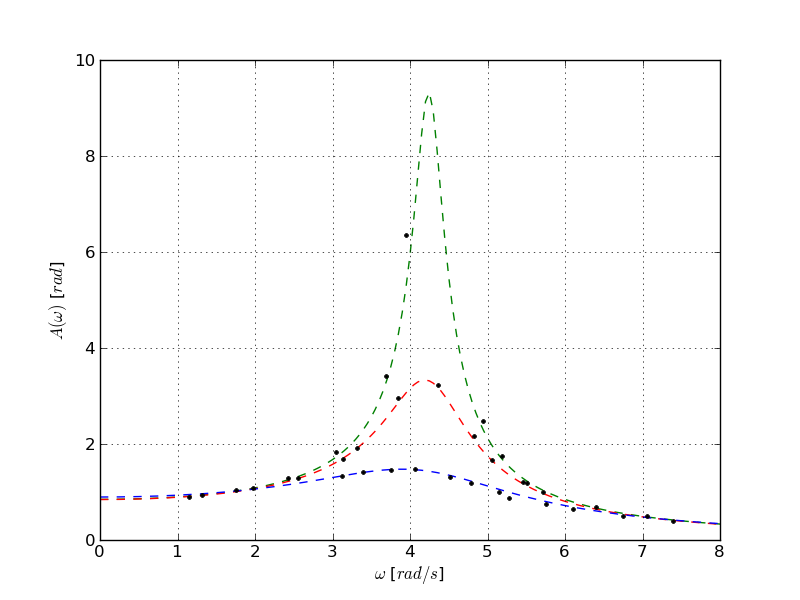
\includegraphics[scale=0.85]{../grafici/risonanza}
\end{center}

Sovvrapponiamo le curve trovate in precedenza, e vediamo verificarsi la condizione di risonanza.
Con l'approssimarsi di $\gamma $ a zero, la curva blu ha infatti $\gamma=1.40\ s^{-1}$, la rossa $\gamma=0.543\ s^{-1}$, la verde $\gamma=0.193\ s^{-1}$,  il valore dell'ampiezza tende a $+\infty$.

\begin{center}
\begin{tabular}{c c}

\begin{tabular}{c|c|c|c}
&$\omega_0\ Libere\ (rad/s) $ & $\omega_0\ Smorzate\ (rad/s) $ & $\omega_0\ Smor. Forzate \ (rad/s) $\\
\midrule
4.80mm&4.27 &4.25 & 4.25 \\
2.80mm&4.27 & 4.30 & 4.26 \\
1.00mm&4.27 &4.29& 4.37 \\
\end{tabular}
&
\begin{tabular}{c|c}
$\gamma_0\ Forzate $ & $\gamma_0\ Smorzate $\\
\midrule
1.40 &1.50\\
0.543 &0.636\\
$\sim 0$ &0.193\\
\end{tabular}
\end{tabular}
\end{center}

Pur trattandosi dello stesso parametro, ricavandolo attraverso interpolazioni e condizioni fisiche diverse, si ottengono valori leggermente differenti. All'aumentare dello smorzamento i valori si discostano maggiormente fra di loro. 


